\documentclass[11pt,a4paper]{article}

\usepackage{lmodern}
\usepackage[T1]{fontenc}
\usepackage[utf8]{inputenc}
\usepackage[margin=1in]{geometry}
\usepackage{amsmath}
\usepackage{graphicx}
\usepackage{booktabs}
\usepackage{float}
\usepackage{caption}
\usepackage[hidelinks]{hyperref}

\captionsetup{font=small,labelfont=bf}
\graphicspath{{figures/}}

\newcommand{\code}[1]{\texttt{\small #1}}

\title{\textbf{Numerical Methods for Large-Scale Ranking Systems}}
\author{%
2105118 \quad 2105119 \quad 2105110 \quad 2105115 \quad 2105107\\[0.4em]
Subsection B2 \\[0.4em]
\normalsize Numerical Analysis Sessional (CSE 402)
}

\date{\today}

\begin{document}

\maketitle

\section*{Summary of Results}

We computed PageRank for a web graph of 281{,}903 pages using four different
numerical methods, and then tried combining two of them to see if we could do better.
Here is what we found:

\begin{itemize}
  \item \textbf{All three exact methods agree.} Power Iteration, Sparse LU and Sparse
        QR gave the same answer to about 14 decimal places.
  \item \textbf{LU was the fastest exact method} at roughly 45 seconds, compared to
        115 seconds for Power Iteration and 584 seconds for QR.
  \item \textbf{Monte Carlo was about 100 times faster} than Power Iteration, but only
        approximate. It still found the top pages correctly.
  \item \textbf{Our hybrid warm start worked.} Seeding Power Iteration with a Monte
        Carlo estimate cut the iteration count from 146 to 141, saving 5 iterations at
        the same accuracy. Section~\ref{sec:hybrid} looks at why the saving was this
        size and how it could be pushed further.
\end{itemize}

\section{What We Planned to Do}

Our project was based on the paper \emph{``Monte Carlo Methods in PageRank
Computation: When One Iteration Is Sufficient''} by Avrachenkov, Litvak, Nemirovsky
and Osipova. The paper claims that a single short random walk from each page is
already enough to produce a useful ranking.

In our proposal we said we would:

\begin{enumerate}
  \item Implement four methods (LU, QR, Power Iteration and Monte Carlo) and
        compare their accuracy and running time.
  \item Try our own extension: give Power Iteration a ``warm start'' by using the
        Monte Carlo result as its starting vector instead of a flat uniform guess. We
        expected this would need fewer iterations and therefore finish faster.
\end{enumerate}

This report covers both, including a closer look at how much the warm start actually
helps and what controls the size of that effect.

\section{Background}

PageRank is based on a simple idea: a page is important if important pages link to it.
If there are $n$ pages, we build a matrix $P$ where
\[
  P_{ji} = \frac{1}{\text{number of outgoing links of page } i}
  \qquad \text{if page } i \text{ links to page } j,
\]
and $0$ otherwise. With a damping factor $d = 0.85$, which is the probability that a
surfer keeps clicking links instead of jumping to a random page, the PageRank vector $r$
satisfies
\begin{equation}
  r = d\,P r + \frac{1-d}{n}\mathbf{1}.
  \label{eq:pagerank}
\end{equation}

\subsection{Two ways to solve it}

\textbf{As a repeated update.} Start with a guess for $r$, put it into the right-hand
side of \eqref{eq:pagerank}, get a new $r$, and repeat until it stops changing. This
is Power Iteration.

\textbf{As a system of linear equations.} Move all the $r$ terms to one side:
\begin{equation}
  A r = b, \qquad A = I - dP, \qquad b = \frac{1-d}{n}\mathbf{1}.
  \label{eq:linsys}
\end{equation}
This is now an ordinary linear system, which we can solve using LU or QR
decomposition. The matrix $A$ is extremely sparse: only about 2.6 million of its
roughly $7.9\times10^{10}$ entries are non-zero.

\subsection{Dangling pages}

Some pages have no outgoing links at all (172 in our dataset). These are called
\emph{dangling} pages, and they break the method: the surfer gets stuck there, so the
probabilities no longer add up to 1.

The textbook fix is to pretend that a dangling page links to every other page. But
that would fill an entire column of $P$ with non-zeros and destroy the sparsity, which
is the only reason these methods are affordable at all. So instead we solve two
systems that share the \emph{same} matrix $A$,
\[
  A x = \frac{1-d}{n}\mathbf{1},
  \qquad
  A y = \frac{d}{n}\mathbf{1},
\]
and then combine them:
\begin{equation}
  r = x + \mu\, y,
  \qquad
  \mu = \frac{\text{sum of } x \text{ over the dangling pages}}
             {1 - \text{sum of } y \text{ over the dangling pages}}.
  \label{eq:dangling}
\end{equation}
Since both systems use the same $A$, only one decomposition is needed. Power Iteration
does not need this trick, since it simply spreads the stuck probability evenly over all
pages at each step.

\section{The Methods We Implemented}

\begin{description}
  \item[Power Iteration.] Repeat \eqref{eq:pagerank} until the change between two
    steps drops below $10^{-12}$.
  \item[Sparse LU.] Factorize $A = LU$ with SciPy's sparse solver, then solve. We use
    its answer as our reference, because it is a direct method (so it does not depend
    on a convergence tolerance the way Power Iteration does) and it was also the
    fastest exact method we measured.
  \item[Sparse QR.] Factorize $A = QR$ with SuiteSparseQR, then solve. We used two
    optimizations here, described in Section~\ref{sec:qr}.
  \item[Monte Carlo.] Send random walkers across the graph and count where they go.
    An \emph{endpoint} method counts only the page where each walk stops. A
    \emph{complete path} method counts every page the walk passes through. Each walk
    stops with probability $1 - d$ at every step.
  \item[Hybrid (our extension).] Run Monte Carlo first to get a rough answer, then
    hand that answer to Power Iteration as its starting vector.
\end{description}

\section{Setup}

\begin{table}[H]
\centering
\caption{Dataset and parameters.}
\begin{tabular}{ll}
\toprule
\textbf{Property} & \textbf{Value} \\
\midrule
Dataset          & \code{web-Stanford.txt} \\
Pages (nodes)    & 281{,}903 \\
Links (edges)    & 2{,}312{,}497 \\
Dangling pages   & 172 \\
Damping factor $d$ & 0.85 \\
Stopping tolerance & $10^{-12}$ \\
Reference answer & Sparse LU \\
Walks per page   & 1 \\
\bottomrule
\end{tabular}
\end{table}

All methods were run on the same machine, so the timings are fair to compare with one
another.

\section{Results}

\subsection{The three exact methods agree}

Power Iteration converged in \textbf{146 iterations}. Table~\ref{tab:top10} lists the
ten highest-ranked pages found by Sparse LU, which we use as our reference
throughout.

\begin{table}[H]
\centering
\caption{Top 10 pages, according to Sparse LU (our reference method).}
\label{tab:top10}
\begin{tabular}{rrl}
\toprule
\textbf{Rank} & \textbf{Node} & \textbf{PageRank (Sparse LU)} \\
\midrule
1  & 89073 & $1.1303\times10^{-2}$ \\
2  & 226411 & $9.2678\times10^{-3}$ \\
3  & 241454 & $8.2973\times10^{-3}$ \\
4  & 262860 & $3.0231\times10^{-3}$ \\
5  & 134832 & $3.0013\times10^{-3}$ \\
6  & 234704 & $2.5717\times10^{-3}$ \\
7  & 136821 & $2.4537\times10^{-3}$ \\
8  & 68889 & $2.4308\times10^{-3}$ \\
9  & 105607 & $2.3910\times10^{-3}$ \\
10  & 69358 & $2.3640\times10^{-3}$ \\
\bottomrule
\end{tabular}
\end{table}

Table~\ref{tab:side} then shows what every other method produced for those same ten
pages, so they can be compared directly against the reference column above.

\begin{table}[H]
\centering
\caption{PageRank of the same top 10 pages, computed by every other method.}
\label{tab:side}
\resizebox{\textwidth}{!}{%
\begin{tabular}{rrcccccc}
\toprule
\textbf{Rank} & \textbf{Node} & \textbf{Power} & \textbf{QR} & \textbf{MC cyclic} & \textbf{MC dangling} & \textbf{MC random} & \textbf{Hybrid} \\
\midrule
1 & 89073 & $1.1303\times10^{-2}$ & $1.1303\times10^{-2}$ & $1.1195\times10^{-2}$ & $1.1146\times10^{-2}$ & $1.1107\times10^{-2}$ & $1.1303\times10^{-2}$ \\
2 & 226411 & $9.2678\times10^{-3}$ & $9.2678\times10^{-3}$ & $9.3472\times10^{-3}$ & $9.2742\times10^{-3}$ & $9.2188\times10^{-3}$ & $9.2678\times10^{-3}$ \\
3 & 241454 & $8.2973\times10^{-3}$ & $8.2973\times10^{-3}$ & $8.3930\times10^{-3}$ & $8.3638\times10^{-3}$ & $8.2772\times10^{-3}$ & $8.2973\times10^{-3}$ \\
4 & 262860 & $3.0231\times10^{-3}$ & $3.0231\times10^{-3}$ & $3.0613\times10^{-3}$ & $2.9531\times10^{-3}$ & $2.9150\times10^{-3}$ & $3.0231\times10^{-3}$ \\
5 & 134832 & $3.0013\times10^{-3}$ & $3.0013\times10^{-3}$ & $3.0933\times10^{-3}$ & $2.9461\times10^{-3}$ & $2.9294\times10^{-3}$ & $3.0013\times10^{-3}$ \\
6 & 234704 & $2.5717\times10^{-3}$ & $2.5717\times10^{-3}$ & $2.5895\times10^{-3}$ & $2.5435\times10^{-3}$ & $2.5207\times10^{-3}$ & $2.5717\times10^{-3}$ \\
7 & 136821 & $2.4537\times10^{-3}$ & $2.4537\times10^{-3}$ & $2.3625\times10^{-3}$ & $2.4240\times10^{-3}$ & $2.5345\times10^{-3}$ & $2.4537\times10^{-3}$ \\
8 & 68889 & $2.4308\times10^{-3}$ & $2.4308\times10^{-3}$ & $2.4902\times10^{-3}$ & $2.3824\times10^{-3}$ & $2.5111\times10^{-3}$ & $2.4308\times10^{-3}$ \\
9 & 105607 & $2.3910\times10^{-3}$ & $2.3910\times10^{-3}$ & $2.2738\times10^{-3}$ & $2.3963\times10^{-3}$ & $2.3576\times10^{-3}$ & $2.3910\times10^{-3}$ \\
10 & 69358 & $2.3640\times10^{-3}$ & $2.3640\times10^{-3}$ & $2.3306\times10^{-3}$ & $2.3605\times10^{-3}$ & $2.3070\times10^{-3}$ & $2.3640\times10^{-3}$ \\
\bottomrule
\end{tabular}%
}
\end{table}

Reading across Table~\ref{tab:side}, the Power Iteration, QR and Hybrid columns are
indistinguishable from the Sparse LU reference at four significant figures. The three
Monte Carlo columns are visibly different but still close, and they never move a page
far from where it belongs. Power Iteration, QR and the Hybrid also reproduce the exact
same top 10 ordering as LU, while the Monte Carlo methods get the top 3 right and
shuffle a few of the lower positions.

This is our main correctness check, and it is a reassuring one. The three methods
work in completely different ways: one repeats a simple update, one factorizes the
matrix into $L$ and $U$, and one factorizes it into $Q$ and $R$. There is no real
chance of all three agreeing to 14 decimal places unless the implementations are
right.

\subsection{Speed and accuracy of every method}

\begin{table}[H]
\centering
\caption{Accuracy and running time. Error is measured against Sparse LU, our reference
method. The $L_1$ error is the sum of absolute differences across all 281{,}903 pages.}
\label{tab:main}
\resizebox{\textwidth}{!}{%
\begin{tabular}{lrrrrr}
\toprule
\textbf{Method} & \textbf{Time (s)} & \textbf{Mean abs.\ error} & \textbf{Max abs.\ error} & \textbf{Mean rel.\ error} & \textbf{$L_1$ error} \\
\midrule
Sparse LU (reference)       & \textbf{45}  & n/a & n/a & n/a & n/a \\
Power Iteration             & 115 & $3.6\times10^{-18}$ & $1.8\times10^{-14}$ & $4.8\times10^{-13}$ & $1.0\times10^{-12}$ \\
Sparse QR                   & 584 & $1.1\times10^{-19}$ & $9.4\times10^{-16}$ & $7.8\times10^{-14}$ & $3.2\times10^{-14}$ \\
\midrule
Monte Carlo, endpoint, cyclic start  & 1.2 & $2.0\times10^{-6}$ & $1.9\times10^{-4}$ & 1.283 & 0.5540 \\
Monte Carlo, complete path, dangling stop & 1.2 & $6.9\times10^{-7}$ & $1.6\times10^{-4}$ & 0.305 & \textbf{0.1957} \\
Monte Carlo, complete path, random start  & 2.4 & $9.6\times10^{-7}$ & $2.0\times10^{-4}$ & 0.574 & 0.2712 \\
\midrule
Hybrid (Monte Carlo warm start) & 122 & $1.5\times10^{-17}$ & $5.9\times10^{-15}$ & $3.0\times10^{-12}$ & $4.3\times10^{-12}$ \\
\bottomrule
\end{tabular}%
}
\end{table}

\begin{figure}[H]
\centering
\begin{minipage}{0.49\textwidth}
  \centering
  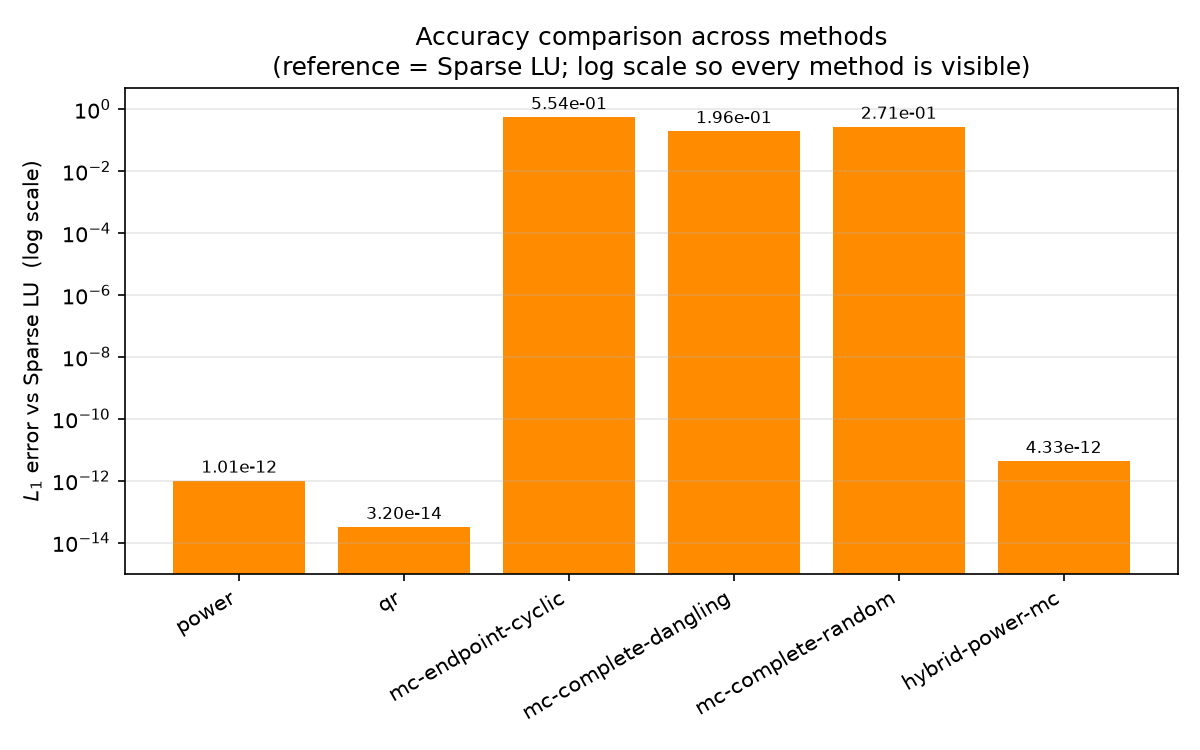
\includegraphics[width=\textwidth]{accuracy_comparison_log.png}
\end{minipage}
\hfill
\begin{minipage}{0.49\textwidth}
  \centering
  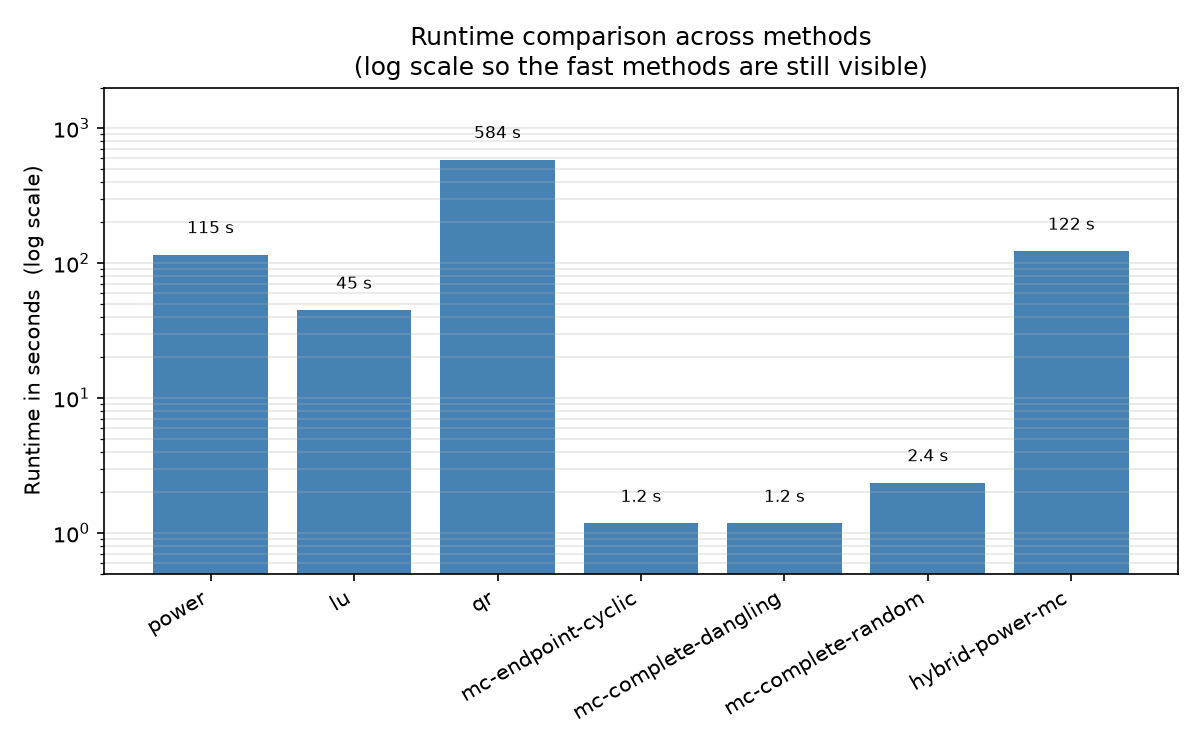
\includegraphics[width=\textwidth]{runtime_comparison_log.png}
\end{minipage}
\caption{Error (left) and running time (right) for every method. Both axes are
logarithmic. This matters: on a normal linear axis the exact methods vanish on the left
chart (their errors are around $10^{-13}$ next to Monte Carlo's $0.55$) and the Monte
Carlo methods vanish on the right chart (about 1 second next to QR's 584). A log axis
spans all of it, so every method shows a real value. The exact number is printed above
each bar. Sparse LU is absent from the left chart because it is the reference, so its
error is exactly zero and cannot be drawn on a log axis.}
\label{fig:acc-rt}
\end{figure}

Three things stand out:

\begin{itemize}
  \item \textbf{LU beat Power Iteration} (about 45 s against 115 s) while being just
        as accurate. This surprised us, since we had assumed the direct method would
        be the slow one on a graph this big.
  \item \textbf{QR was by far the slowest}, at about 584 seconds, roughly 13 times
        slower than LU, even though it solves exactly the same system.
        Section~\ref{sec:qr} explains why.
  \item \textbf{The complete-path Monte Carlo method was about three times more
        accurate} than the endpoint method ($L_1$ error $0.196$ against $0.554$) for
        about the same cost. This makes sense: a complete-path method uses information
        from every page the walker visits, while an endpoint method throws all of that
        away and keeps only the last page.
\end{itemize}

\subsection{Where the Monte Carlo error actually is}

\begin{figure}[H]
\centering
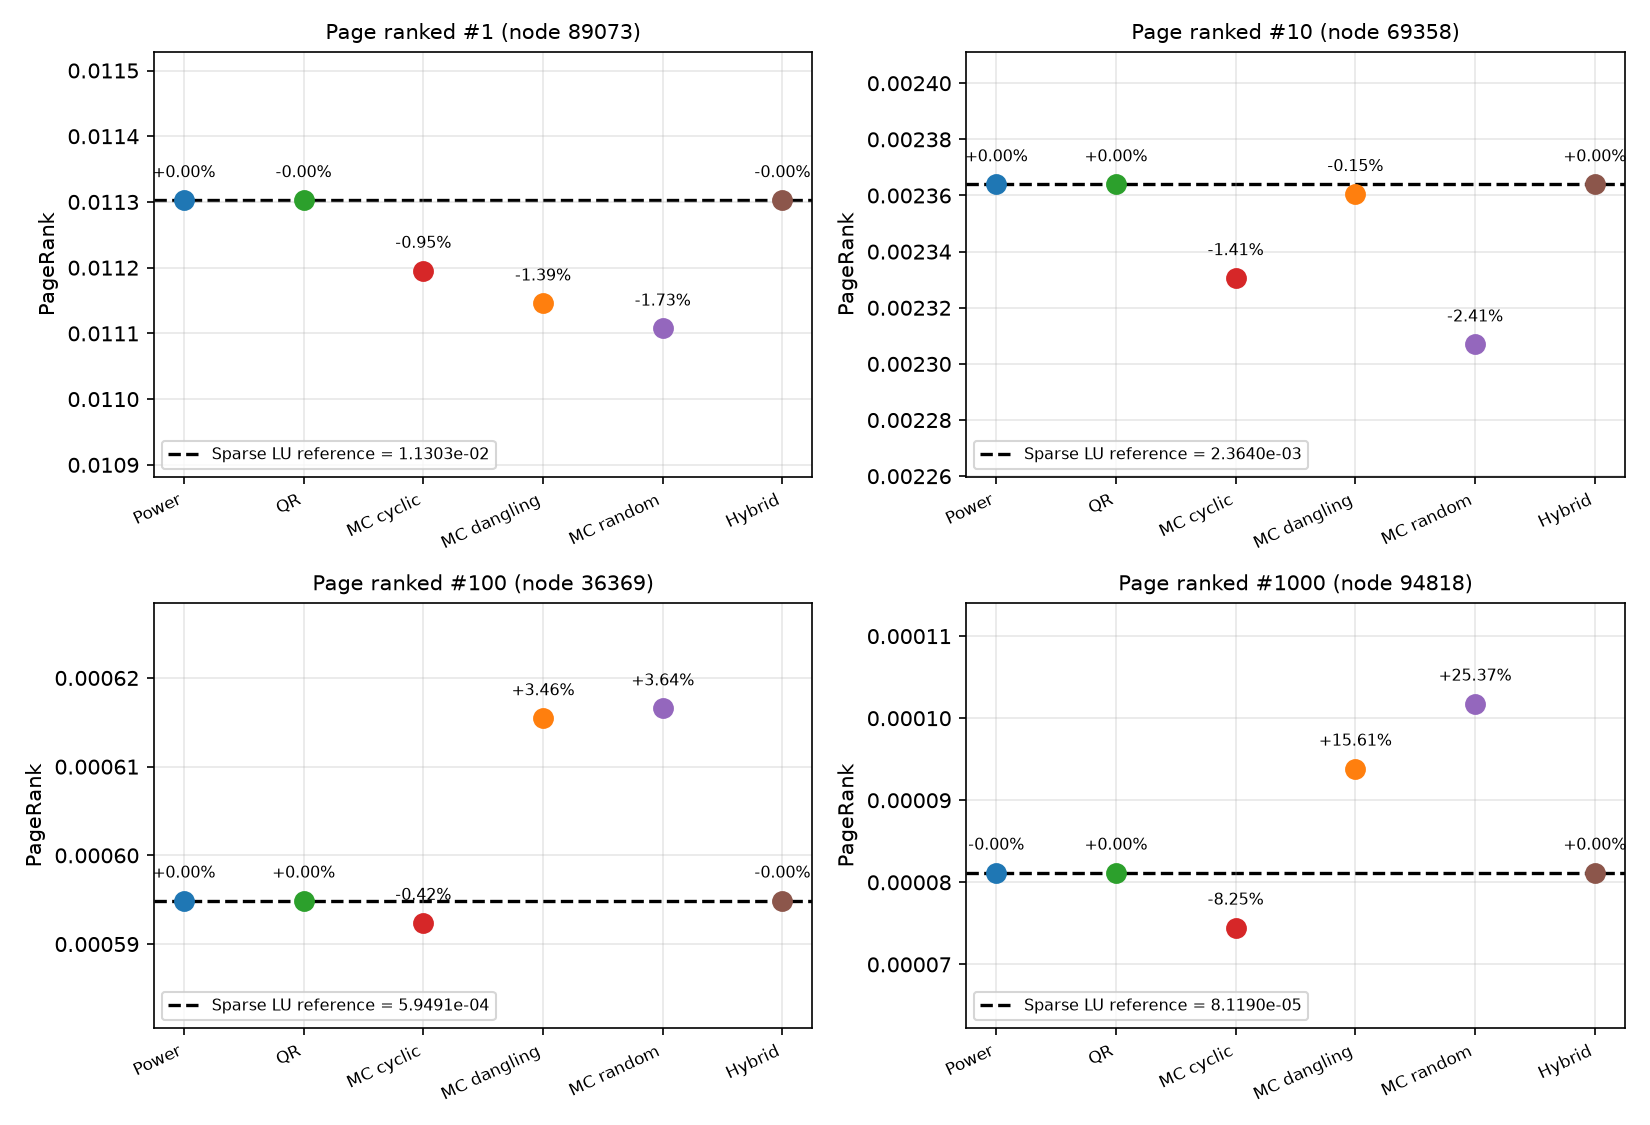
\includegraphics[width=\textwidth]{method_comparison.png}
\caption{Every method compared against the Sparse LU reference, for the pages ranked
1st, 10th, 100th and 1000th. The dashed line in each panel is LU's value, and the
percentage above each point is how far that method lands from it. Power Iteration, QR
and the Hybrid sit exactly on the reference line in all four panels. The three Monte
Carlo methods miss by about 1 to 2\% at the top of the ranking, and the gap widens
sharply further down.}
\label{fig:ci}
\end{figure}

Figure~\ref{fig:ci} makes the split very clear. The two direct methods and the
Hybrid land on the reference line to within rounding at every position we checked. The
Monte Carlo methods behave quite differently depending on where in the ranking we
look:

\begin{center}
\begin{tabular}{lrrrr}
\toprule
\textbf{Method} & \textbf{Rank 1} & \textbf{Rank 10} & \textbf{Rank 100} & \textbf{Rank 1000} \\
\midrule
MC endpoint, cyclic            & $-0.95\%$ & $-1.41\%$ & $-0.42\%$ & $-8.25\%$ \\
MC complete path, dangling     & $-1.39\%$ & $-0.15\%$ & $+3.46\%$ & $+15.61\%$ \\
MC complete path, random start & $-1.73\%$ & $-2.41\%$ & $+3.64\%$ & $+25.37\%$ \\
\bottomrule
\end{tabular}
\end{center}

\noindent
At the very top of the ranking the Monte Carlo estimates are within about 1 to 2\% of
LU, which is easily good enough to identify the important pages. By rank 1000 the same
methods are off by 8 to 25\%.

The same effect shows up in Table~\ref{tab:main}. For the best Monte Carlo method the
average \emph{absolute} error is tiny ($6.9\times10^{-7}$), but the average
\emph{relative} error is about 31\%. These two numbers disagree because they are
dominated by different pages:

\begin{itemize}
  \item \textbf{Important pages} have large PageRank values and are visited by many
        walkers, so they are estimated accurately.
  \item \textbf{Unimportant pages} have PageRank values close to $1/n$. A walker may
        visit such a page once, or never. If the true value is $4\times10^{-6}$ and we
        estimate $8\times10^{-6}$, the absolute error is negligible but the relative
        error is 100\%.
\end{itemize}

Since there are far more unimportant pages than important ones, they dominate the
average relative error. This is exactly why the paper's claim works in practice: if
the goal is to find the important pages, one walk per page is enough, because the
error ends up in the places where it does not matter.

\subsection{Why QR was so much slower than LU}
\label{sec:qr}

Both LU and QR are direct methods solving the same system \eqref{eq:linsys}, so the
13-fold difference in running time needs an explanation. The reason is a well-known
problem called \textbf{fill-in}.

The matrix $A$ is very sparse. But the factors produced by a decomposition are not:
they gain non-zero entries in positions where $A$ had none. Web graphs make this
especially bad, because a few ``hub'' pages link to tens of thousands of other pages.
When the algorithm eliminates a hub, it connects all of that hub's neighbours to each
other at once, and the effect spreads.

QR suffers from this more than LU does. It needs roughly twice as many arithmetic
operations, it cannot take advantage of the fact that $A$'s sparsity pattern is nearly
symmetric, and it has to store the Householder reflectors that build $Q$. The result
is a much larger factor and a much longer runtime.

We applied two optimizations to make QR finish at all:

\begin{enumerate}
  \item \textbf{COLAMD ordering.} SuiteSparseQR can reorder the columns before
        factorizing, to reduce fill-in. The default setting tries several different
        orderings and keeps the best one, which is very expensive on a graph this
        large. We fixed it to COLAMD, a single cheap heuristic. This does not change
        the answer, only how long it takes to compute.
  \item \textbf{One factorization for both right-hand sides.} The dangling correction
        \eqref{eq:dangling} needs two solves with the same matrix $A$. Instead of
        calling the solver twice, we pass both right-hand sides together in one call.
        This halves the number of factorizations, which is the expensive part.
\end{enumerate}

Even with these, QR needed about 584 seconds and a large amount of memory. Our
conclusion is that QR is a valid method for this problem but a poor choice for it: it
gives no accuracy advantage over LU and costs 13 times more.

\subsection{The hybrid warm start reduced the iteration count}
\label{sec:hybrid}

\begin{table}[H]
\centering
\caption{Plain Power Iteration versus our Monte Carlo warm start.}
\begin{tabular}{lrrr}
\toprule
\textbf{Method} & \textbf{Iterations} & \textbf{Time (s)} & \textbf{$L_1$ error} \\
\midrule
Power Iteration (flat starting guess $1/n$) & 146 & 115 & $1.0\times10^{-12}$ \\
Hybrid (Monte Carlo starting guess)         & 141 & 122 & $4.3\times10^{-12}$ \\
\bottomrule
\end{tabular}
\end{table}

The warm start worked. Starting from the Monte Carlo estimate, Power Iteration
reached the same $10^{-12}$ tolerance in \textbf{141 iterations} instead of 146, so the
better starting guess saved \textbf{5 iterations}. The hybrid also lands on the same
answer as the reference, matching Sparse LU to $4.3\times10^{-12}$, so nothing is given
up in accuracy.

This confirms the core of our hypothesis: a rough sampled ranking really is a better
place to begin than a flat uniform guess, and the method notices the difference.

\medskip
\noindent\textbf{Why was the saving only 5 iterations?}

Power Iteration shrinks its error by roughly the same factor at every step, and that
factor is the damping constant $d = 0.85$. This happens no matter where the iteration
starts. Every step just multiplies whatever error is left by about $0.85$.

So a better starting guess lowers the error we begin with, but it does not make the
method converge any \emph{faster per step}. To reach a tolerance of $10^{-12}$ the
method still has to push the error down through roughly 12 orders of magnitude at a
fixed rate, and starting a bit closer only removes a few steps from the front.

\medskip
\noindent\textbf{Could it be made to work?}

The obvious thing to vary next is the number of walks per page. We used only one walk
per page for the warm start, which is the cheapest Monte Carlo estimate available and
also the least accurate one. With more walks the starting guess would sit closer to
the true answer, and it should save more than 5 iterations.

There is a balance to strike, since more walks also take longer to generate. From
Table~\ref{tab:main} the Monte Carlo methods run in about 1 to 2 seconds, while a
single Power Iteration step costs roughly $115/146 \approx 0.8$ seconds. Sampling is
therefore cheap relative to an iteration, which suggests there is a sweet spot worth
searching for. Finding it is the clear next experiment, and it is what we would try
first if we carried this project further.

Looking back, working out the size of this effect was the most useful thing we
learned. It is tempting to treat \emph{starting closer to the answer} and
\emph{converging faster} as the same idea, but for a method with a fixed convergence
rate they are quite different, and seeing that play out in our own measurements made
the distinction much clearer than reading about it would have.

\section{What We Learned}

\begin{enumerate}
  \item \textbf{All three exact methods agree to about 14 decimal places}, which
        confirms our implementations are correct.
  \item \textbf{LU was the fastest exact method} (about 45 s versus 115 s for Power
        Iteration). In our proposal we assumed LU would only be usable on small
        graphs; for a graph of this size that assumption was wrong.
  \item \textbf{QR was the slowest method of all} (about 584 s), even though it solves
        the same system as LU and gives the same answer. The reason is fill-in, which
        affects QR much more than LU. So ``direct methods do not scale'' is too simple
        a statement, because it depends on which factorization is used.
  \item \textbf{Monte Carlo is a good trade-off.} One walk per page found the
        important pages correctly in about 1\% of the time, and the error landed
        mostly on unimportant pages.
  \item \textbf{Our hybrid warm start reduced the iteration count} from 146 to 141,
        confirming that a sampled starting vector beats a flat one. The saving is
        limited by the fact that a starting guess cannot change the convergence
        \emph{rate}, which is fixed at $d = 0.85$. Using more walks per page should
        widen the gap, and that is the experiment we would run next.
\end{enumerate}

\subsection*{Limitations}

All timings come from a single run on one machine, and Monte Carlo results vary a
little with the random seed, and Figure~\ref{fig:ci} shows how much. We also tested only
one graph size. Running the same experiments on graphs of several different sizes would
show more clearly how each method scales as the graph grows, which was one of the
measurements listed in our proposal.


\end{document}
